% Chebotarev as a dartboard: the group G partitioned into conjugacy
% classes; the chance of a random prime's Frobenius class landing in
% each class is proportional to its size.
% Source: book/tex/alg-NT/frobenius.tex (§ Chebotarev density
% theorem) — asy.
\documentclass[border=2mm]{standalone}
\usepackage{tikz}
\usepackage{amssymb}
\usepackage{amsmath}
\begin{document}
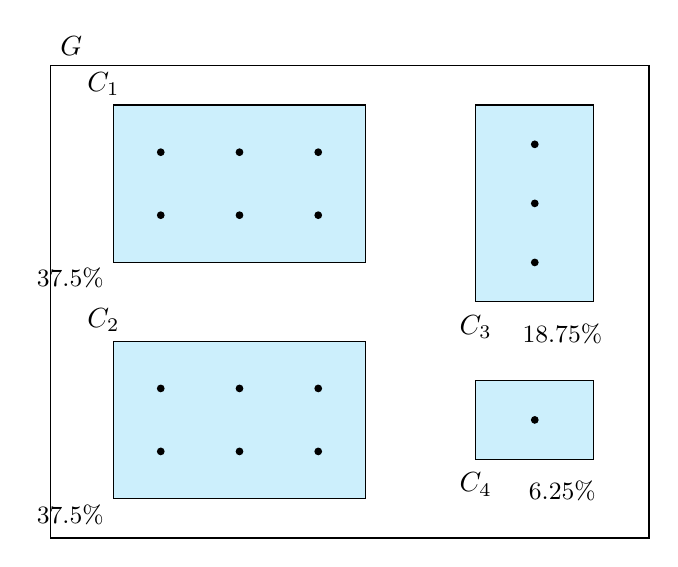
\begin{tikzpicture}
  \draw (-3.4,-3) rectangle (4.2,3);
  \node[anchor=south west] at (-3.4,3) {$G$};
  \filldraw[fill=cyan!20, draw=black] (-2.6,0.5) rectangle (0.6,2.5);
  \filldraw[fill=cyan!20, draw=black] (-2.6,-2.5) rectangle (0.6,-0.5);
  \filldraw[fill=cyan!20, draw=black] (2,0) rectangle (3.5,2.5);
  \filldraw[fill=cyan!20, draw=black] (2,-2) rectangle (3.5,-1);
  \foreach \x in {-2,-1,0} {
    \fill (\x,1.9) circle (1.4pt);
    \fill (\x,1.1) circle (1.4pt);
    \fill (\x,-1.9) circle (1.4pt);
    \fill (\x,-1.1) circle (1.4pt);
  }
  \node[anchor=east] at (-2.6,0.3) {\small $37.5\%$};
  \node[anchor=east] at (-2.6,-2.7) {\small $37.5\%$};
  \node[anchor=south east] at (-2.4,2.5) {$C_1$};
  \node[anchor=south east] at (-2.4,-0.5) {$C_2$};
  \fill (2.75,2.0) circle (1.4pt);
  \fill (2.75,1.25) circle (1.4pt);
  \fill (2.75,0.50) circle (1.4pt);
  \fill (2.75,-1.5) circle (1.4pt);
  \node[anchor=north] at (2,-0.05) {$C_3$};
  \node[anchor=north] at (3.1,-0.15) {\small $18.75\%$};
  \node[anchor=north] at (2,-2.05) {$C_4$};
  \node[anchor=north] at (3.1,-2.15) {\small $6.25\%$};
\end{tikzpicture}
\end{document}
